\documentclass[11pt]{article}

\usepackage[margin=1in]{geometry}
\usepackage{amsmath,amssymb,mathtools,bm}
\usepackage{graphicx}
\usepackage{booktabs}
\usepackage{placeins}
\usepackage[colorlinks=true,linkcolor=blue,citecolor=blue,urlcolor=blue]{hyperref}

\graphicspath{{../figures/}}

% --- macros (shared with the companion analytic paper) ---
\newcommand{\rs}{\bm{r}_s}
\newcommand{\rw}{\bm{r}_w}
\newcommand{\Del}{\bm{\Delta}}
\newcommand{\nhat}{\hat{\bm{n}}}
\newcommand{\uhat}{\hat{\bm{u}}}
\newcommand{\Bhat}{\hat{\bm{B}}}
\newcommand{\Nfp}{N_{\mathrm{fp}}}
\newcommand{\eps}{\varepsilon}
\newcommand{\epseff}{\eps_{\mathrm{eff}}}
\newcommand{\half}{\tfrac{1}{2}}
\newcommand{\NWL}{\mathrm{NWL}}
\newcommand{\dd}{\,\mathrm{d}}
\newcommand{\iso}{\mathrm{iso}}

\title{\bfseries A Native Spin-Polarized Fusion Neutron Source for OpenMC:
Stellarator Wall-Loading, the Rate--Steering Trade-off, and Where Monte-Carlo
Transport Is Necessary}

\author{
Thaddaeus Kiker\textsuperscript{1,2}
\and
Ethan Peterson\textsuperscript{3}
\\[4pt]
\small \textsuperscript{1}Department of Astronomy, Columbia University, New York, NY, USA\\
\small \textsuperscript{2}Fusion Research Center, Columbia University, New York, NY, USA\\
\small \textsuperscript{3}Plasma Science and Fusion Center, Massachusetts Institute of Technology, Cambridge, MA, USA
}
\date{\today}

\begin{document}
\maketitle

\begin{abstract}
\noindent
Spin polarization of deuterium--tritium fuel both enhances the fusion rate and makes the
$14.1$~MeV neutron emission anisotropic about the local magnetic field, so the first-wall
neutron load of a polarized reactor depends on the plasma shape, the field geometry, and
the polarization mix together. We build the first \emph{native, on-the-fly} spin-polarized
fusion neutron \emph{source} in a production Monte-Carlo transport code (OpenMC): a
thread-safe sampler that draws the polarized birth direction exactly, for an arbitrary
polarization mix and an arbitrary \emph{local} field direction evaluated per birth point.
Because the local field is required at every position, the source is realized as a
\texttt{StellaratorSource} that draws births and the unit field $\Bhat$ from a verified
three-dimensional VMEC equilibrium---the first equilibrium-rigorous, polarized stellarator
source, and the first stellarator source of any kind in OpenMC. We give the emission kernel
and its separation into a birth-direction distribution and a scalar rate factor, an exact
stratified sampler with a closed-form inverse-CDF cross-checked against rejection, and a
degeneracy-free frame rotation; we verify the sampler in isolation to $0.3\%$ per bin, and
verify the transported loads against the analytic free-streaming NWL where the two must
agree ($\le1.8\%$ on a real published QA equilibrium, with a $4$--$6\%$ inboard residual
that we identify by construction as the analytic point-patch limit, not a defect of the
source). We then use the source to do what the free-streaming and analytic pictures
cannot. First, \emph{scattering dilutes the geometric steering by a factor of
$\sim\!3$}: the $\pm40\%$ inboard contrast of the free-streaming limit realizes as only
$\pm13$--$15\%$ through a real blanket, because backscattered neutrons return as a
direction-blind diffuse flux. Second, restoring the reactivity separates what the three
polarization modes buy---the $+50\%$-rate mode compounds the center-stack load to
$1.70\times$, while the equal-rate parallel mode relieves it to $0.85\times$ at no cost to
power or to the tritium breeding ratio. Third, on conformal first walls of real
quasi-symmetric stellarators, peaking-optimal polarization lowers the peaking factor only
modestly (e.g.\ $1.78\to1.49$): the load peak is a narrow near-field spike that angular
redistribution cannot move, so polarization is a strong \emph{local} actuator but a weak
\emph{global} flattener---a conclusion an independent differentiable analytic method
reaches as well. The source is available for both tokamak- and stellarator-class
equilibria and provides a verified foundation for polarized-fuel reactor neutronics.
\end{abstract}

\section{Introduction}
\label{sec:intro}

Spin-polarized fusion (SPF) aligns the reactant nuclear spins to raise the D--T reaction
cross section by up to $50\%$ and to redirect the angular distribution of the fusion
products~\cite{kulsrud1982,parisi2024,schwartz2025}. The neutron carries $80\%$ of the
D--T energy, so the redistribution of the $14.1$~MeV neutrons directly reshapes the
first-wall neutron load---the quantity that sets the blanket, shield, and material
lifetimes of a reactor, and the second of the two central problems of fusion neutronics
alongside tritium self-sufficiency~\cite{lyytinen2024}---and the optimal polarization
choice is a system decision that must be made against that load~\cite{schwartz2025,lion2022}.
Scoping studies quantify the load through the neutron wall load (NWL), the first-flight
neutron current through a wall patch weighted by the neutron energy; it omits scattering
but is inexpensive and is therefore the natural object for design
iteration~\cite{lion2022,schwartz2025}. A reactor calculation, however, needs the
transported load: the volumetric heating and breeding that follow once the anisotropic
birth distribution is carried through a real, scattering blanket.

The polarized neutron emission is not isotropic. For a chosen mixture of deuteron and
triton spin projections the differential cross section is a fixed combination of two
angular shapes referred to the local field direction $\Bhat$: a $\sin^2\theta$ shape that
peaks perpendicular to $\Bhat$ and a $\tfrac14+\tfrac34\cos^2\theta$ shape that peaks
parallel to it, where $\theta$ is the angle between the emitted neutron and
$\Bhat$~\cite{schwartz2025}. Because $\Bhat$ follows the magnetic geometry, the wall load
of a polarized plasma is a convolution of the emission kernel, the field, and the source
distribution over the plasma volume against the wall geometry---and evaluating the
emission at the \emph{local} field direction is precisely what a shape parametrization
cannot supply and a solved equilibrium can.

\paragraph{Prior work, and the gap.}
Two complementary routes evaluate the polarized NWL convolution. The first is analytic. For
an axisymmetric device the toroidal source integral over a planar ring reduces to
incomplete elliptic integrals, giving a fast, automatically differentiable NWL suited to
shape and polarization optimization~\cite{schwartz2025}; a companion analytic development
(\S\ref{sec:companion}) restores this closed form perturbatively for weakly shaped QA
boundaries, valid while the geometric non-axisymmetry is small, and is free-streaming by
construction. The second route is Monte-Carlo, and here the closest prior work must be
placed carefully. \cite{bae2025} performed the first polarized-source neutronics in
OpenMC, but by \emph{precomputing} a static point-source cloud for one fixed spherical-
tokamak scheme; the emission directions are baked in ahead of the run rather than sampled
on the fly in the local field frame, which is what a spatially varying stellarator field
requires. Parametric stellarator neutronics in production codes has meanwhile focused on
the \emph{geometry}: \cite{lyytinen2024} scan blanket thickness for a HELIAS in Serpent2
with a neutron source ``integrated \dots\ as a user-defined source routine based on the
MCNP code''---a ported, isotropic routine, not one derived from the equilibrium's own
volume element---and parametric tokamak plasma sources exist in OpenMC as
well~\cite{peterson_tokamaksource}, but are unpolarized and axisymmetric. What does not yet
exist is a \emph{native, general, on-the-fly polarized} source that both samples the
correct anisotropic emission in the local field frame and is driven by a real
three-dimensional equilibrium so that it applies to stellarators. We build it.

\paragraph{Contributions and organization.}
We contribute (i) the first native, on-the-fly polarized fusion source in a production MC
code, and its verification, including an exact self-consistency identity in the
polarization parameter; (ii) \texttt{StellaratorSource}, equilibrium-rigorous polarized
emission from a gated VMEC equilibrium, the first such source in OpenMC; and (iii) the use
of that source to establish results the free-streaming and analytic pictures structurally
cannot---the $\sim\!3\times$ scattering dilution of steering, the rate-versus-steering
trade-off among the polarization modes, and the finding that polarization is a strong local
but weak global actuator of the wall load, the last cross-validated by an independent
analytic method. The paper is organized as a ladder of models, each used at the fidelity
that isolates one effect. Section~\ref{sec:source} states the emission kernel and its
birth-direction/rate separation. Section~\ref{sec:mc} gives the exact sampler, the
equilibrium birth-position and field models, and the OpenMC realization.
Section~\ref{sec:sampler} verifies the sampler in isolation. Section~\ref{sec:validation}
cross-validates the transported free-streaming loads against the analytic method on a real
published QA equilibrium, and Section~\ref{sec:pointpatch} identifies the one residual as
the analytic point-patch limit. Section~\ref{sec:transport} turns on scattering and reports
the dilution of the steering; Section~\ref{sec:rate} restores the reactivity and the
rate-versus-steering trade-off; Section~\ref{sec:conformal} evaluates conformal-wall loads
for real stellarators and the local-versus-global result; and
Section~\ref{sec:conformalscatter} transports the source through a conformal multi-material
blanket for the volumetric flux and heating. Section~\ref{sec:companion}
describes the analytic companion and the division of labour, Section~\ref{sec:limitations}
bounds the claims, and Section~\ref{sec:summary} summarizes.

\section{The spin-polarized emission source}
\label{sec:source}

We follow the parameterization of Ref.~\cite{schwartz2025}. Let the deuteron spin
projection fractions be $d_+,d_0,d_-$ and the triton fractions $t_+,t_-$. The three
collision-mode fractions are
\begin{equation}
a=d_+t_++d_-t_-,\qquad b=d_0,\qquad c=d_+t_-+d_-t_+,\qquad a+b+c=1,
\label{eq:abc}
\end{equation}
with the unpolarized fuel at $a=b=c=\tfrac13$.\footnote{Our $(a,b,c)$ are Schwartz's
collision-mode fractions~\cite{schwartz2025}; they should not be confused with the
identically-named vector/tensor polarization parameters used by Bae~\cite{bae2025}, whose
scheme has no separate ``mode $c$.''} The differential cross section, referred to
the local field direction $\Bhat$, is
\begin{equation}
\frac{\dd\sigma}{\dd\Omega}=\frac{\sigma_0}{2\pi}\left[\tfrac34\,a\,\sin^2\theta
+\left(\tfrac23 b+\tfrac13 c\right)\left(\tfrac14+\tfrac34\cos^2\theta\right)\right],
\qquad \cos\theta=\Bhat\cdot\hat{\bm\Delta},
\label{eq:dsdo}
\end{equation}
where $\hat{\bm\Delta}$ is the emitted neutron direction and $\sigma_0$ is the cross
section in the $S=\tfrac32$ combined-spin state. Integrating Eq.~\eqref{eq:dsdo} over the
sphere gives the total rate $\sigma_{\rm tot}=\sigma_0\,\eta$ with
$\eta=a+\tfrac23 b+\tfrac13 c$; the unpolarized value is $\tfrac23\sigma_0$, pure $a$
(mode A) is $\sigma_0$ (a $50\%$ enhancement), and pure $c$ (mode C) is $\tfrac13\sigma_0$.
Modes B and C share the same angular shape $\tfrac14+\tfrac34\cos^2\theta$ and differ only
in rate: the emission of a polarized plasma is controlled by two angular functions, not
three. (Mode C is therefore \emph{not} isotropic---a common misassignment---but shares its
directionality with mode B while emitting at half the rate.)

The essential structure for sampling is that the \emph{birth direction} and the
\emph{total rate} separate. Collecting the two angular shapes,
\begin{equation}
I(\theta)=w_\perp\sin^2\theta+w_\parallel\!\left(\tfrac14+\tfrac34\cos^2\theta\right),
\qquad w_\perp=\tfrac34 a,\quad w_\parallel=\tfrac23 b+\tfrac13 c,
\label{eq:I}
\end{equation}
the normalized birth-direction density is $p(\theta,\phi)=I(\theta)/\!\int I\dd\Omega$ with
$\phi$ uniform, and it depends only on $(w_\perp,w_\parallel)$. The overall rate factor
$\eta$ multiplies the spatial source strength and does not enter the direction sampling.
Keeping these two concerns separate is the central design choice: the sampler draws a
correctly shaped direction for any $(a,b,c)$, and $\eta$ is applied, if absolute loads are
wanted, as a scalar weight on the birth-position distribution. It is convenient to
summarize the direction by a single parameter, writing the normalized intensity as
$w(\theta)\propto1+a_2\,P_2(\cos\theta)$ with $a_2\in[-1,+1]$, where $a_2=-1$ is the pure
perpendicular shape, $a_2=+1$ the pure parallel shape, and $a_2=0$ isotropic; because $P_2$
enters linearly, the wall load is exactly linear in $a_2$, a fact we exploit for
verification in \S\ref{sec:conformal}. For the free-streaming cross-checks the direction is
all that matters, and the birth energy is taken monoenergetic at $14.1$~MeV; a
Ballabio-broadened Gaussian at a specified ion temperature is available for physical runs
and is irrelevant to the angular verification.

\section{Monte-Carlo realization}
\label{sec:mc}

\paragraph{Exact stratified direction sampling.}
Because Eq.~\eqref{eq:I} is a nonnegative combination of two shapes, we sample the birth
direction by stratification: with probability $W_\perp/(W_\perp+W_\parallel)$ draw from
the $\sin^2\theta$ shape, otherwise from the $\tfrac14+\tfrac34\cos^2\theta$ shape, where
$W_\perp=w_\perp\!\int\!\sin^2\theta\dd\Omega=\tfrac{8\pi}{3}w_\perp$ and
$W_\parallel=w_\parallel\!\int(\tfrac14+\tfrac34\cos^2\theta)\dd\Omega=2\pi w_\parallel$
are the solid-angle-integrated weights. This is an exact draw from the mixture and makes
per-mode verification trivial. Each shape is sampled by a closed-form inverse-CDF in
$x=\cos\theta$: the $\sin^2\theta$ shape has marginal $\propto\sin^3\theta$ and is inverted
by the trigonometric solution of the depressed cubic $x^3-3x+2(1-2\xi)=0$; the
$\tfrac14+\tfrac34\cos^2\theta$ shape has marginal $\propto\tfrac14+\tfrac34x^2$ and is a
cubic in $x$ as well. Each inverse-CDF is cross-checked against an independent rejection
sampler (envelope $\propto\sin\theta$, acceptance $\tfrac23$) to a two-sample
Kolmogorov--Smirnov tolerance, so the root selection in the cubic is verified rather than
assumed. The azimuth $\phi$ is uniform on $[0,2\pi)$. The sampler holds no mutable state:
every derived weight is fixed at construction and the sampling methods are constant, so the
concurrent, per-thread calls OpenMC makes are race-free, and randomness comes only from
OpenMC's own counter-based stream.

\paragraph{Local-to-global rotation.}
The sampled direction is expressed in a frame with $\hat{\bm z}_{\rm loc}\parallel\Bhat$
and rotated to global Cartesian by a Gram--Schmidt construction that avoids the
$\Bhat\parallel\hat{\bm z}$ degeneracy: the reference axis is whichever of
$\hat{\bm x},\hat{\bm y},\hat{\bm z}$ is least aligned with $\Bhat$, and
$\hat{\bm x}_{\rm loc}=\mathrm{normalize}(\hat{\bm e}_{\rm ref}-(\hat{\bm e}_{\rm ref}\!\cdot\!\Bhat)\Bhat)$,
$\hat{\bm y}_{\rm loc}=\Bhat\times\hat{\bm x}_{\rm loc}$. The resulting global direction is
unit to machine precision and, tested with a random non-axis $\Bhat$, leaves an isotropic
local distribution isotropic---the check that the rotation carries no bias.

\paragraph{Birth positions and the equilibrium field.}
The birth-position model is pluggable. For the free-streaming cross-checks the plasma is
represented by constant-$(\rho,\vartheta)$ filaments on a set of scaled flux surfaces,
sampled uniformly in the toroidal angle and weighted by the arc-length Jacobian and a model
emissivity $W(\rho)\propto\rho^2$; the same filaments are the source loops of the analytic
method, so the two calculations share the source exactly and the comparison isolates the
transport treatment. For the equilibrium-driven runs of \S\ref{sec:conformal}, births are
drawn from a three-dimensional VMEC~\cite{hirshman1983} equilibrium with the physically
correct weight, reactivity times the metric Jacobian $\sqrt{g}$, and the unit field is
reconstructed from the equilibrium as
$\bm B=B^u\partial_\vartheta\bm x+B^v\partial_\zeta\bm x$ with $\Bhat=\bm B/|\bm B|$. The
producer hard-gates its invariants---an independent divergence-theorem volume must match
the VMEC volume to better than $1.5\times10^{-2}$, and $\sqrt{g}$ must be single-signed---so
the spatial distribution and the field direction the source consumes are verified, not
assumed. This upgrades the parametric tokamak-source
pattern~\cite{peterson_tokamaksource} on four axes: real equilibrium geometry, correct
$\sqrt{g}$ volumetric weighting, genuine three-dimensionality, and the local field
direction that makes the polarized emission well posed in the first place.

\paragraph{OpenMC source and transport.}
The sampled births are handed to OpenMC~\cite{romano2015} either through a compiled
custom-source shared library or as a pre-sampled source bank written to an HDF5 file and
read back as a fixed source. For the free-streaming cross-checks the vessel interior is
void and the walls are vacuum boundaries, so each neutron streams in a straight line from
its birth point until it crosses a surface and is tallied; the wall load is a
surface-current tally binned poloidally. This ray-traced transport makes no point-patch or
$1/D^2$ approximation---a neutron reaches a wall patch if and only if its sampled trajectory
does---which is the property that the analytic comparison below tests. The same source, run
with a material first wall and blanket rather than a void, gives the transported load
(\S\ref{sec:transport}--\ref{sec:conformal}); on the conformal geometries the first wall is
a CAD surface imported through DAGMC~\cite{dagmc}.

\section{Verification of the sampler}
\label{sec:sampler}

The sampler is verified before any geometry is introduced. Drawing $2\times10^6$
directions per mode about a fixed $\Bhat=\hat{\bm z}$ and histogramming in equal
$\cos\theta$ bins, the sampled directionality---the ratio of the mode density to the
isotropic density in each bin---reproduces the normalized kernels
$\tfrac32\sin^2\theta$ (mode A) and $2(\tfrac14+\tfrac34\cos^2\theta)$ (mode B/C) to
better than $0.3\%$ per bin, and the mean directionality of each polarized mode is
$1.0000$, confirming that the stratified draw is normalized to unit emission exactly
(Table~\ref{tab:sampler}). A $\chi^2$ test against the analytic $p(\cos\theta)$ for
$\{$unpolarized, A, B, C, mixed$\}$ and a two-sample KS test of inverse-CDF against
rejection close the sampler verification; the isotropic and rotation-isotropy checks are
flat as required. This isolates the sampler from every subsequent test: any later
discrepancy is geometric, not a defect of the angular draw.

\begin{table}[t]
\centering
\caption{Sampler self-test: sampled directionality $A/\iso$ and $B/\iso$ per
$\cos\theta$ bin against the exact normalized kernels, and the mode means. The sampled
kernels match to $0.3\%$ and integrate to unit emission ($1.0000$), so the direction draw
is exact independent of any geometry.}
\label{tab:sampler}
\begin{tabular}{ccccc}
\toprule
$\cos\theta$ & $A/\iso$ (MC) & $\tfrac32\sin^2\theta$ & $B/\iso$ (MC) & $2(\tfrac14+\tfrac34\cos^2\theta)$ \\
\midrule
$-0.95$ & $0.146$ & $0.146$ & $1.857$ & $1.854$ \\
$-0.15$ & $1.467$ & $1.466$ & $0.535$ & $0.534$ \\
$+0.05$ & $1.491$ & $1.496$ & $0.505$ & $0.504$ \\
$+0.85$ & $0.414$ & $0.416$ & $1.582$ & $1.584$ \\
\midrule
mean & $1.0000$ & $1$ & $1.0000$ & $1$ \\
\bottomrule
\end{tabular}
\end{table}

\section{Cross-validation against the analytic method}
\label{sec:validation}

The decisive test is that the Monte-Carlo source reproduces the analytic free-streaming
NWL where the analytic method is itself exact. We compare on a shared square-cross-section
torus wall, so that all non-axisymmetry lives in the source and the wall is common to both
calculations, and we compare the wall directionality $A/\iso$ and $B/\iso$---the ratio of
the polarized load to the isotropic load on each wall---which cancels the source
normalization and isolates the polarized steering. The analytic side is a pure-numpy
free-streaming quadrature that evaluates the loop geometry and field directly at the
Gauss--Legendre nodes with the true shaped-loop visibility and the inner-cylinder
occlusion; it is gated at run time against the companion \texttt{anarr\'ima} quadrature
and matches it to $10^{-12}$, so it is the analytic method's own reference, only faster. We
use a genuine published equilibrium: because the standard published QA configurations are
all strongly shaped (a survey of DESC examples gives $\epseff\approx1$--$2.6$ at a tight
wall), we mined the QUASR stellarator database~\cite{quasr} for a gentle one without the
bulk download---pulling its single tabulated catalogue ($3.7\times10^5$ devices), filtering
to quasi-axisymmetry, ranking by a metadata proxy that correlates with the geometric
excursion (correlation $0.94$), and computing the exact $\epseff$ of a shortlist from the
VMEC boundary spectra. The gentlest is a $\Nfp=3$ QA of aspect ratio $6.7$, which at the
validation wall has $\epseff\approx0.43$---four times more shaped than an idealized toy and,
unlike it, near the edge of the analytic method's convergent band
(Fig.~\ref{fig:quasrgeom}). The published QAs proper sit well beyond that edge: at their
native $\epseff\approx2.3$ the analytic series diverges and even the fixed-node exact
quadrature fails, disagreeing with the reference by $\sim\!34\%$ and returning unphysical
negative loads from the near-singular grazing integrand---so the strongly shaped
configurations are Monte-Carlo-only, and it is the gentle mined equilibrium that permits a
cross-check at all.

On this configuration the Monte-Carlo and analytic directionalities agree to $\le1.8\%$ on
the outboard, floor, and ceiling walls, with the poloidal profiles tracked to correlation
$0.7$--$0.99$; the inner (inboard) wall shows a larger, $4$--$6\%$ residual
(Table~\ref{tab:quasr}, Fig.~\ref{fig:quasr}). The inboard wall is where the analytic
companion's own controlling parameter $\epseff$ is largest---it is local and peaks where
the standoff is smallest---so a departure there, on the most strongly curved wall of the
most strongly shaped case, is exactly where one expects the free-streaming analytic to be
most stressed. The next section shows that this residual is a limit of the analytic method,
not of the Monte-Carlo source.

\begin{figure}[t]
\centering
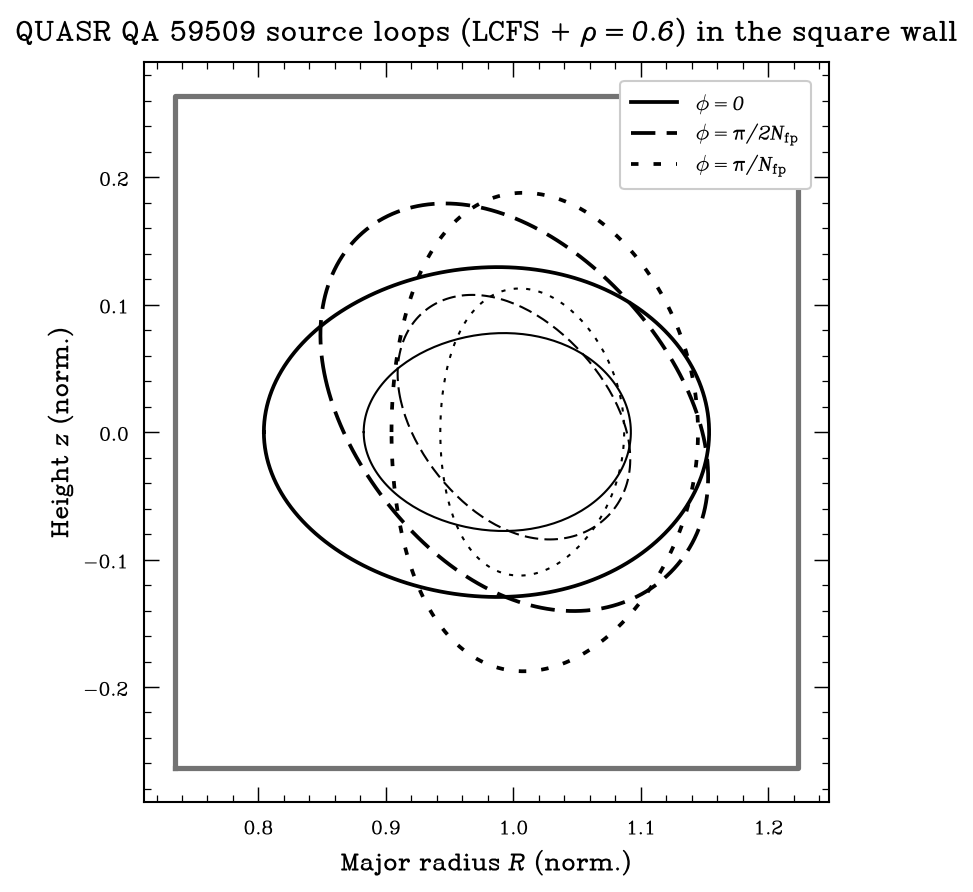
\includegraphics[width=0.60\linewidth]{quasr59509_geometry.png}
\caption{Source loops of the real QUASR QA equilibrium (device 59509, $\Nfp=3$): the
last-closed and an interior flux surface at several toroidal cuts, showing the rotating,
strongly shaped cross section, inside the square-cross-section wall used for the
cross-check.}
\label{fig:quasrgeom}
\end{figure}

\begin{table}[t]
\centering
\caption{Real QUASR QA ($\epseff\!\approx\!0.43$): directionality $A/\iso$, $B/\iso$ as a
ratio of total wall loads, Monte-Carlo vs analytic. Outboard/floor/ceiling agree to
$\le1.8\%$; the inboard wall carries the $4$--$6\%$ residual analyzed in
\S\ref{sec:pointpatch}.}
\label{tab:quasr}
\small
\begin{tabular}{lcccc}
\toprule
wall & $A$ MC & $A$ an & $B$ MC & $B$ an \\
\midrule
outboard & $0.833$ & $0.848$ & $1.165$ & $1.152$ \\
floor    & $1.048$ & $1.057$ & $0.955$ & $0.943$ \\
ceiling  & $1.043$ & $1.057$ & $0.954$ & $0.943$ \\
\textbf{inboard}  & $1.248$ & $1.199$ & $0.755$ & $0.801$ \\
\bottomrule
\end{tabular}
\end{table}

\begin{figure}[t]
\centering
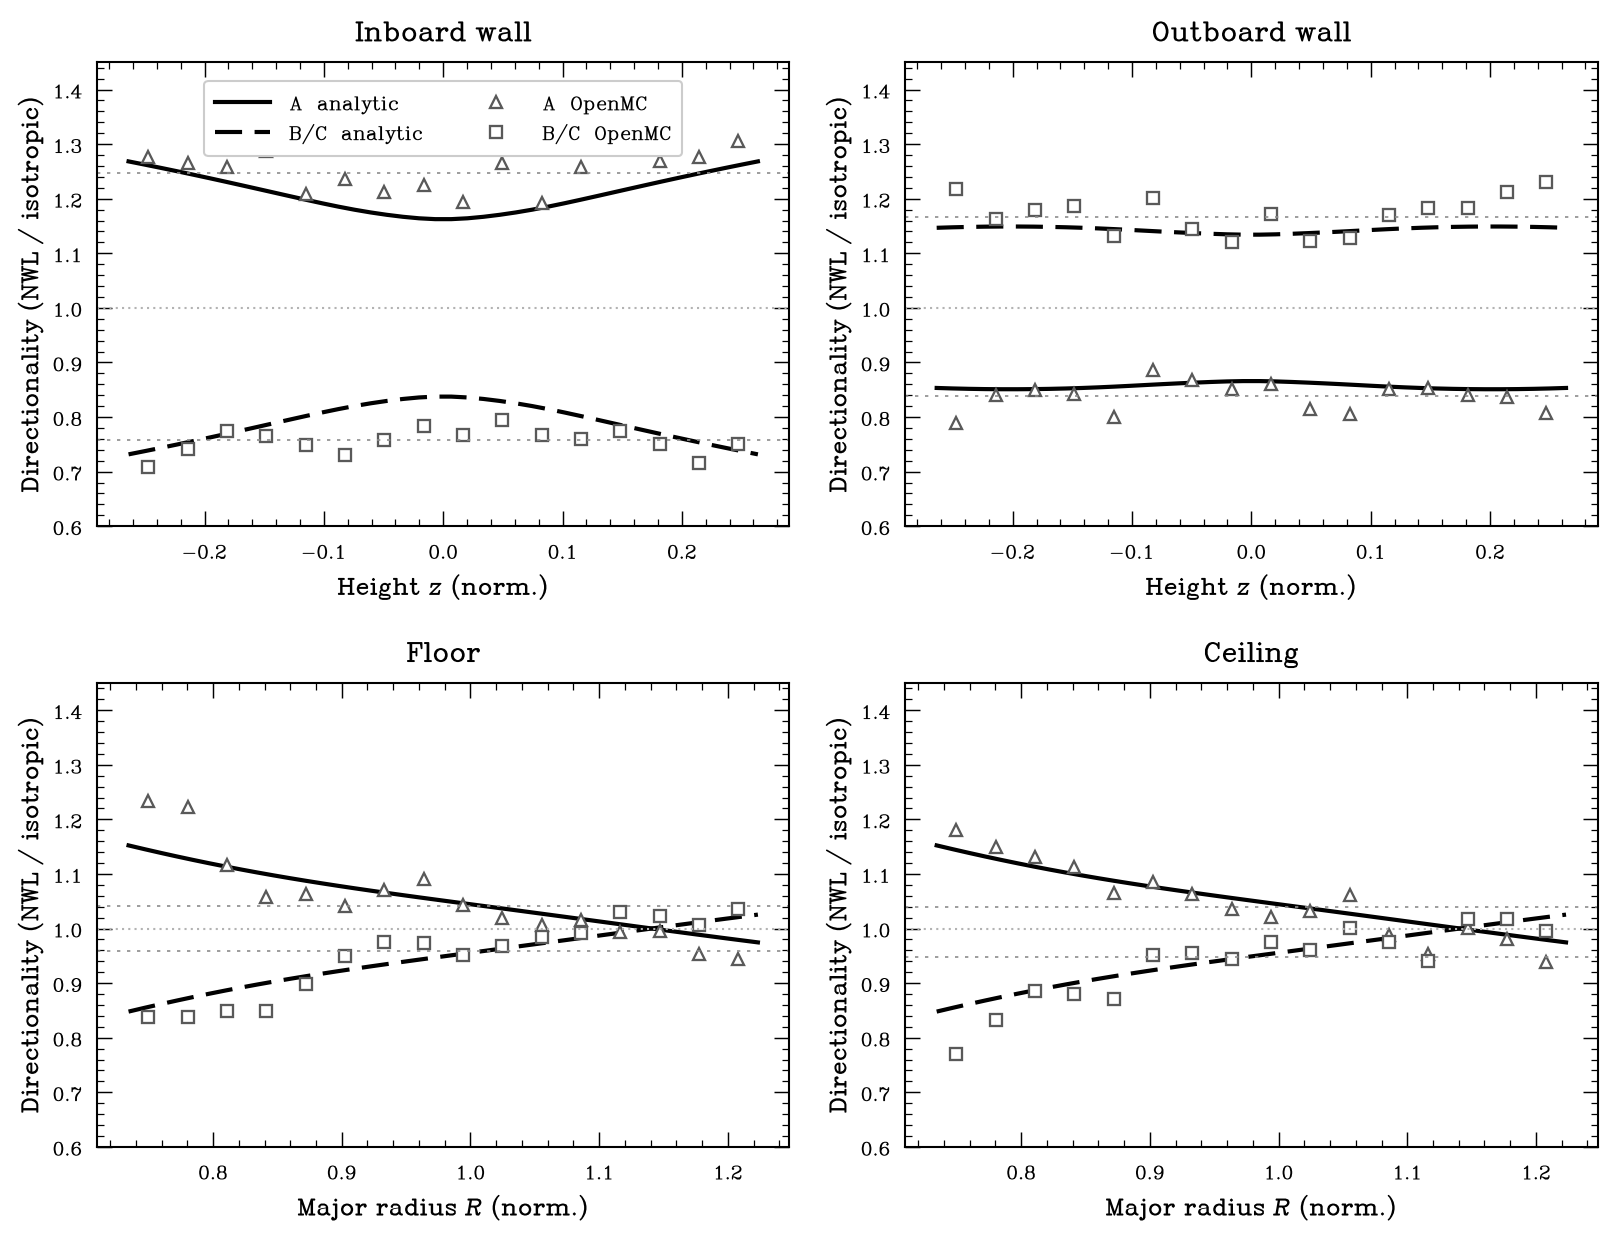
\includegraphics[width=\linewidth]{quasr59509_directionality.png}
\caption{Free-streaming directionality $A/\iso$ (mode A) and $B/\iso$ (mode B/C) around
each wall of the square torus for the real QUASR QA equilibrium ($\epseff\approx0.43$):
the analytic point-patch flux integral (curves) and the OpenMC ray-traced source
(markers). The outboard, floor, and ceiling walls overlay; the inboard wall tracks the
poloidal shape with the $4$--$6\%$ offset. Per-panel vertical scales because the walls
differ by an order of magnitude in poloidal curvature.}
\label{fig:quasr}
\end{figure}

\section{The point-patch limit of the analytic method}
\label{sec:pointpatch}

The inboard residual is small but coherent, and its cause is worth establishing because it
maps the boundary between the two methods. We first eliminate the Monte-Carlo source as the
cause, then reproduce the effect by direct construction. The residual is not the direction
sampler, which reproduces the kernels exactly (\S\ref{sec:sampler}); not the analytic
quadrature, which matches \texttt{anarr\'ima} to $10^{-12}$; not the visibility model,
since using the true shaped-loop sub-arcs with inner-cylinder occlusion rather than a
mean-radius arc removes an unrelated outboard error but leaves the inboard value unchanged;
not the field model, since the analytic and Monte-Carlo evaluations call the identical
$\Bhat$, which cannot by itself open a gap between them; and not a near-field effect, since
moving the wall outward from a gap of $0.4\,a$ to $0.7\,a$ leaves the offset unchanged
($0.036\to0.034$). What does change it is the plasma shaping---the gentle case agrees on
the inboard wall, the strongly shaped one does not---so the effect is a coupling of the
source shaping to the wall geometry that the two methods treat differently.

The one geometric approximation in the analytic NWL is that each wall patch is a point: the
emission kernel is evaluated along the single line of sight from the source to the patch
centre, whereas a patch on a curved wall subtends a finite solid angle over which the
kernel varies, and the ray-traced Monte-Carlo resolves it. To exhibit this in isolation we
strip the problem to a single shaped filament with a tunable shaping amplitude $s$, emitting
the kernel about a purely toroidal field onto bare inner and outer cylinders, and evaluate
the wall directionality two ways: the analytic point-patch flux integral, and an exact
ray/surface intersection of the same sampled births. Here the sampler, field, and occlusion
are all trivially correct, so $s$ is the only variable. The result (Fig.~\ref{fig:barecyl})
is decisive: at $s=0$ the point-patch integral is exact (agreement to $0.002$, the
statistical floor), and as $s$ increases the discrepancy grows as $s^2$, about three times
faster on the convex inner cylinder than on the concave outer, reaching $\sim10\%$ on the
inner wall at the strongest shaping. This reproduces both the inboard-specific location and
the shaping scaling of the full-equilibrium residual, and identifies it unambiguously as
the point-patch treatment of the flux integral on a strongly curved wall---a property of
the analytic method, with the geometry-exact, sampler-exact Monte-Carlo source as the
reference. It is precisely the strongly shaped, strongly curved regime that motivates a
transport calculation, and to which we now turn.

\begin{figure}[t]
\centering
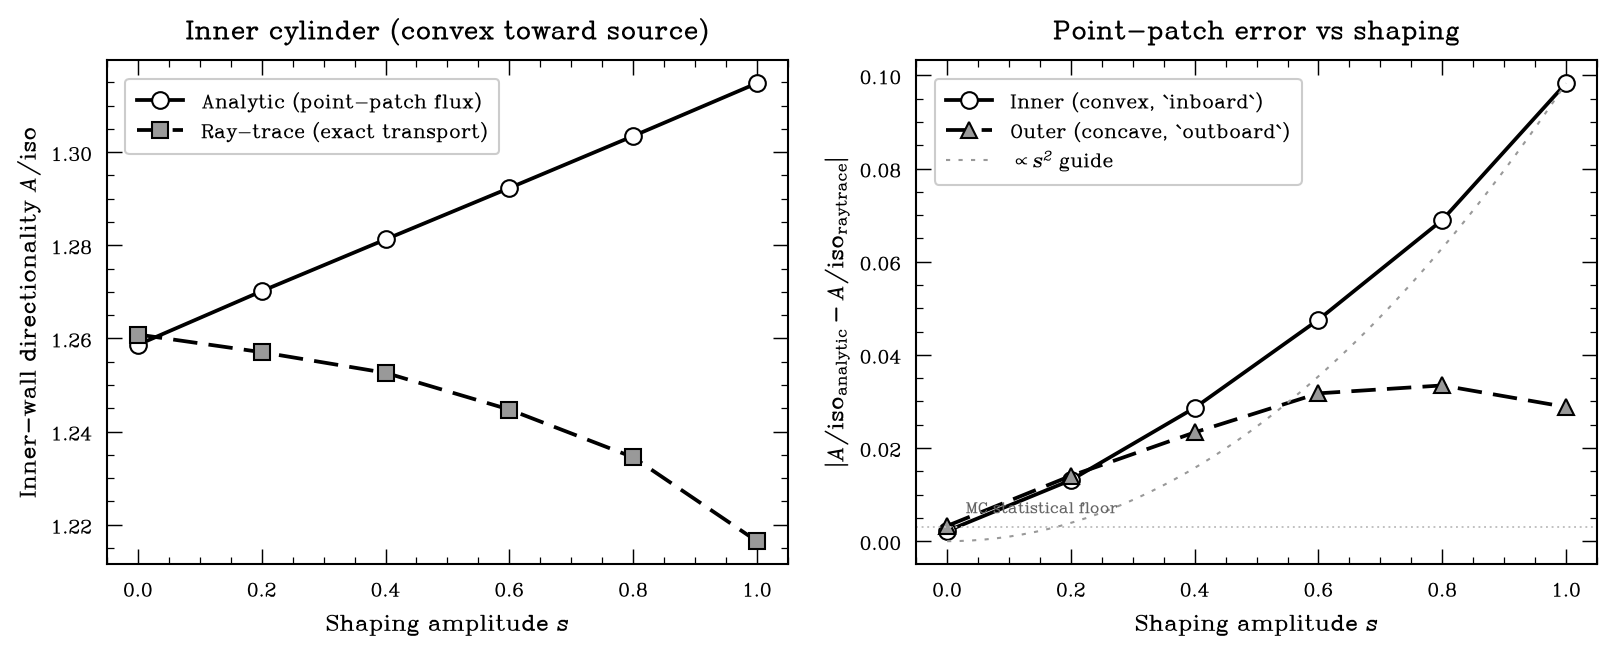
\includegraphics[width=\linewidth]{bare_cylinder_demo.png}
\caption{Single-filament demonstration that the inboard residual is the analytic
point-patch limit. Left: inner-wall directionality $A/\iso$ from the analytic point-patch
flux integral and from exact ray-tracing of the same births, versus the shaping amplitude
$s$; coincident for an axisymmetric source ($s=0$) and diverging as $s$ grows. Right: the
analytic$\leftrightarrow$ray-trace discrepancy versus $s$ for the convex inner (inboard)
and concave outer (outboard) cylinders, with an $s^2$ guide.}
\label{fig:barecyl}
\end{figure}

\section{Transport on a realistic wall: scattering dilutes the steering}
\label{sec:transport}

The free-streaming cross-checks certify the source; the reason to have a Monte-Carlo source
is what the analytic method cannot do, and the first of these is neutron transport. To
obtain a first, clean estimate of how much scattering erodes the geometric steering, we
isolate the transport effect by measuring it in the same axisymmetric square-torus geometry
used for validation---holding the wall fixed and changing only the material, so that any
departure from the free-streaming steering is attributable to scattering alone rather than
to a change of shape, and the radially layered blanket gives every neutron a well-defined
path through the layers for an unambiguous energy and breeding accounting. Replacing the
void interior and vacuum walls with an ARC-class layered blanket---a $1$~mm tungsten first
wall, $1$~cm of Fe-9Cr structural steel, a $1$~cm beryllium multiplier, and $40$~cm of
FLiBe breeder---turns the first-flight NWL into the transported flux and heating that a
reactor blanket actually sees. This box-torus estimate isolates the dilution factor; the
definitive transported load on the conformal geometry, whose free-streaming limit is
validated above (Fig.~\ref{fig:confxcheck}), follows by running the identical source and
blanket on the DAGMC conformal wall, and is expected to carry the same dilution. The polarized angular
emission enters this calculation only through the source; everything downstream is standard
neutron transport, so the anisotropy is carried into the volumetric loads without further
approximation. As an anchor, reducing every layer density by $10^{-4}$ (mean free path
$\gg$ device) recovers the validated free-streaming steering to within statistics---the A
mode raising the inboard load by $+40.0\%$ and lowering the outboard by $-19.5\%$, against
the free-streaming $+39\%/-21\%$---so the layered model and the compiled source are correct
with the full geometry.

The transported result is that \emph{scattering dilutes the steering by a factor of
$\sim\!3$} (Fig.~\ref{fig:dilution}). With the real FLiBe/Be blanket, neutrons that enter
the wall scatter back into the cavity as a diffuse, direction-blind flux, washing out the
directional contrast: the A mode's inboard enhancement falls from $+40\%$ to $+13.2\%$ and
its outboard suppression from $-20\%$ to $-9.2\%$, while the B/C mode's inboard relief falls
from $-40\%$ to $-15.0\%$ and its outboard rise from $+19\%$ to $+9.0\%$. The parallel mode
still relieves the inboard center stack, but by $\sim\!15\%$, not the $\sim\!41\%$ the
geometric picture suggests. This is exactly the correction the free-streaming and analytic
methods structurally cannot provide, and it is a caution for the field: geometric and
analytic steering numbers, ours included, are optimistic by a factor of $\sim\!3$ once a
scattering blanket is present. (The energy bookkeeping confirms an active blanket: the
FLiBe absorbs $91.4\%$ of the deposited energy and the tungsten first wall only $\sim\!0.1\%$,
with total heating $0.87\times$ the birth energy and a down-scattered keV tail that is
absent in the free-streaming model and that drives the low-energy breeding.)

\begin{figure}[t]
\centering
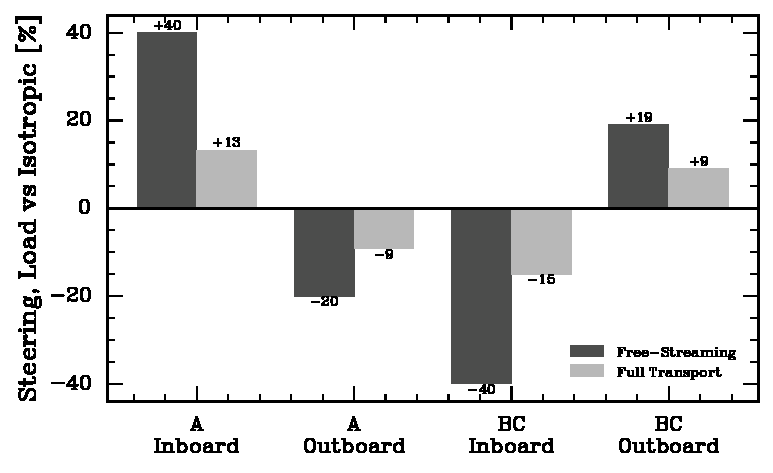
\includegraphics[width=0.68\linewidth]{fig_dilution.pdf}
\caption{Scattering dilutes the geometric steering by $\sim\!3\times$. The free-streaming
inboard/outboard contrast (dark) versus the same quantity transported through a real
layered blanket with scattering on (light), for the perpendicular (A) and parallel (B/C)
modes. The $\pm40\%$ geometric contrast realizes as only $\pm13$--$15\%$ at the wall.}
\label{fig:dilution}
\end{figure}

\section{The rate-versus-steering trade-off}
\label{sec:rate}

The cross-checks above held the fusion rate fixed to isolate directionality. Restoring it
at fixed fuel density---the neutron yield scales with the rate factor $\eta=a+\tfrac23
b+\tfrac13 c$ of Eq.~\eqref{eq:dsdo}, which carries the Kulsrud reactivity
enhancement~\cite{kulsrud1982} the constant-rate comparisons normalized away---separates
what the three polarization modes buy (Fig.~\ref{fig:rate}, Table~\ref{tab:rate}). The A
mode delivers $+50\%$ fusion power and $+49\%$ absolute tritium, but because its emission
is perpendicular to $\Bhat$ it steers neutrons toward the inboard midplane, so the
center-stack load \emph{compounds} to $1.70\times$ (rate times inboard steering)---excellent
for power, hard on the center stack. The B mode carries the same power and breeding as
unpolarized fuel but relieves the center-stack load to $0.85\times$: it buys the directional
benefit at no rate penalty, and is the sweet spot for wall-load control. The C mode halves
both power and breeding but gives the lowest absolute center-stack load ($0.42\times$),
worthwhile only if the center-stack load is the single binding constraint. Crucially, the
tritium breeding ratio \emph{per neutron} is nearly mode-independent ($1.144$--$1.155$), so
the rate boost breeds proportionally more tritium and self-sufficiency is preserved:
polarization redistributes and rescales the load without endangering breeding adequacy.

\begin{table}[t]
\centering
\caption{Absolute quantities at fixed fuel density, relative to unpolarized fuel $=1$
(scattering on). The A mode's rate boost compounds with its inboard steering; the B mode
buys steering at no rate cost; the TBR per neutron is mode-independent.}
\label{tab:rate}
\small
\begin{tabular}{lccccc}
\toprule
mode & rate $\eta$ & fusion rate & center-stack load & outboard load & TBR/neutron \\
\midrule
unpolarized & $0.667$ & $1.00$ & $1.00$ & $1.00$ & $1.149$ \\
A & $1.000$ & $1.50$ & $\mathbf{1.70}$ & $1.36$ & $1.144$ \\
B & $0.667$ & $1.00$ & $\mathbf{0.85}$ & $1.09$ & $1.155$ \\
C & $0.333$ & $0.50$ & $0.42$ & $0.55$ & $1.155$ \\
\bottomrule
\end{tabular}
\end{table}

\begin{figure}[t]
\centering
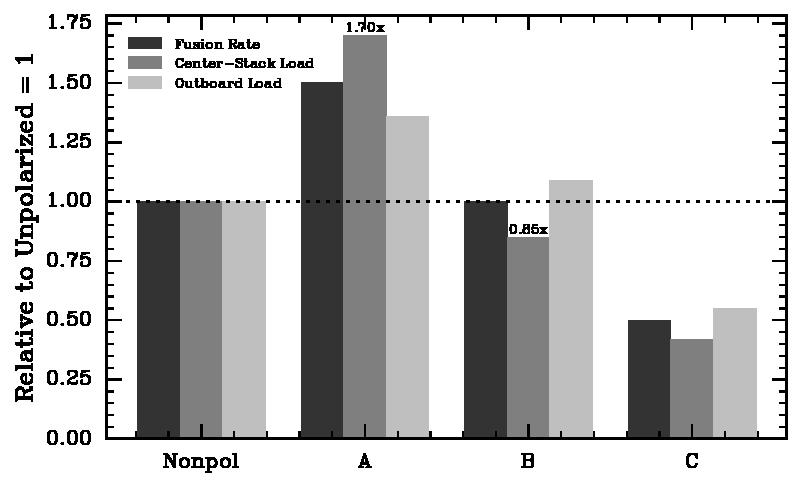
\includegraphics[width=0.68\linewidth]{fig_rate_steering.pdf}
\caption{The rate-versus-steering trade-off (relative to unpolarized $=1$). The A mode buys
power but compounds the center-stack load to $1.70\times$; the B mode buys inboard relief
($0.85\times$) at no rate cost; the C mode halves everything. The rate boost lives in a
different spin state than the center-stack steering.}
\label{fig:rate}
\end{figure}

\section{Conformal-wall loads: a strong local, weak global actuator}
\label{sec:conformal}

The steering results above use a box-torus for a clean scattering and rate accounting; we
now place the polarized source on the conformal first wall of a real stellarator, the
geometry a reactor would actually build. For each of fifteen quasi-symmetric QUASR
equilibria we take the VMEC last-closed surface, offset it outward by $0.30\,a$ along its
poloidal normal, mesh it as a DAGMC first wall~\cite{dagmc}, and free-stream the polarized
\texttt{StellaratorSource} onto it, capturing wall crossings and binning them into a
$(\vartheta,\phi)$ neutron-load map (three million crossings per mode). Because the load is
exactly linear in the polarization parameter $a_2$, the perpendicular and parallel maps
satisfy $\NWL_{\perp}+\NWL_{\parallel}=2\,\NWL_{\rm unpol}$ bin by bin---an exact
self-consistency identity requiring no analytic reference, which the transported maps
confirm to the few-percent Monte-Carlo level and which we use as an in-situ correctness
check on the whole equilibrium-to-map pipeline.

Before drawing physics from these maps we validate the source free-streaming \emph{on the
conformal geometry itself}, so that the cross-check is not limited to the axisymmetric
square torus of \S\ref{sec:validation}. On the gentle QA (device 59509,
$\epseff\approx0.43$) we evaluate the analytic point-patch free-streaming directionality
$A/\iso$ and $B/\iso$ on the same $(\vartheta,\phi)$ conformal wall grid the ray-traced
OpenMC source was binned onto, using the local field $\Bhat$ at each source voxel and
front-facing visibility. The two agree closely (Fig.~\ref{fig:confxcheck}): the per-bin
correlation is $0.91$, the global mean directionality matches to $\le1.2\%$
($A/\iso$ analytic $1.027$ vs Monte-Carlo $1.018$; $B/\iso$ $0.973$ vs $0.985$), and by
region the agreement is $1.6\%$/$2.3\%$ inboard and $0.5\%$/$0.6\%$ outboard, with the
expected sign---mode A enhances the inboard load and suppresses the outboard, mode B/C the
mirror. The source therefore reproduces the free-streaming NWL on the real conformal wall,
not only in the axisymmetric limit, and the residual is the same shaping-driven point-patch
effect isolated in \S\ref{sec:pointpatch} (small here, at $\epseff\approx0.43$; it grows on
the strongly shaped devices, which is why they are Monte-Carlo-only).

\begin{figure}[t]
\centering
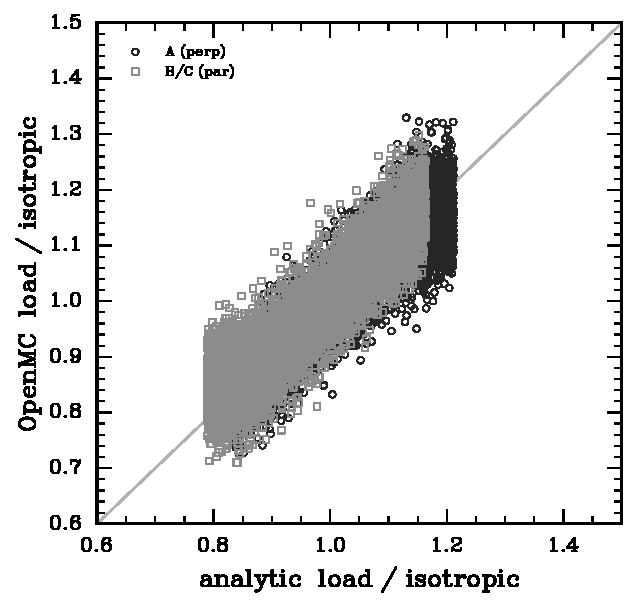
\includegraphics[width=0.52\linewidth]{fig_conformal_xcheck.pdf}
\caption{Free-streaming cross-check \emph{on the conformal wall} (device 59509): analytic
point-patch NWL directionality versus the ray-traced OpenMC \texttt{StellaratorSource}, per
wall bin, for modes A (perp) and B/C (par). The two agree to $0.5$--$2.3\%$ by region
(per-bin correlation $0.91$), validating the source free-streaming on the real
three-dimensional geometry, not only on the axisymmetric square torus.}
\label{fig:confxcheck}
\end{figure}

Scanning $a_2\in[-1,1]$ for the polarization that minimizes the peaking factor
$\mathrm{PF}=\max\NWL/\overline{\NWL}$, we find the optimum is device-specific (parallel for
most devices, perpendicular for a few) but the achievable global flattening is uniformly
modest across the fifteen: peaking-optimal polarization lowers the peaking factor by
$0$--$16\%$, with a median of only $4\%$ (for the most improved device, $1.78\to1.49$;
Fig.~\ref{fig:map}), even though the same polarization commands $40$--$70\%$ swings in the
\emph{local} load between the perpendicular and parallel extremes. The reason is
structural: the peaking factor is set by a narrow near-field spike---the wall's closest
approach to the plasma, a few tenths to a few percent of the wall area---and angular
redistribution reshapes the broad load but cannot move that spike. Polarization is
therefore a strong local actuator and a weak global flattener of the wall load. The proper
use of SPF steering is not to reduce global peaking but to tailor the fluence locally, for
instance to relieve a lightly shielded port or a maintenance-critical panel; the global
peaking is a geometry problem that wall shaping, not polarization, must solve.

It is natural to ask whether the modest, device-specific benefit can be predicted from a
cheap geometric descriptor, so that the transport calculation could be skipped in a design
scan. Across the fifteen devices it cannot (Fig.~\ref{fig:predictor}). Pure-plasma shape
metrics---the non-axisymmetric shaping amplitude of the boundary and a nematic order
parameter of its normals---do not correlate with the steering benefit (Spearman
$\rho=-0.19$ and $+0.40$ respectively, neither significant at $n=15$), consistent with the
line-of-sight integration acting as a low-pass filter that removes the high-harmonic shape
content from the wall signal. The best predictor is a transport-free isotropic
$1/D^2$ peaking proxy---essentially the available headroom, since a device with a larger
geometric hot spot has more to gain---but even it is only borderline
($\rho=+0.53$, $p\approx0.05$), and a spuriously strong correlation seen on the first five
devices ($\rho=+0.90$) regressed toward this value as the sample grew. The practical
conclusion reinforces the paper's thesis: the polarization steering benefit is weak, device
specific, and not forecastable from plasma shape, so it must be evaluated per device by the
transport calculation the source provides.

\begin{figure}[t]
\centering
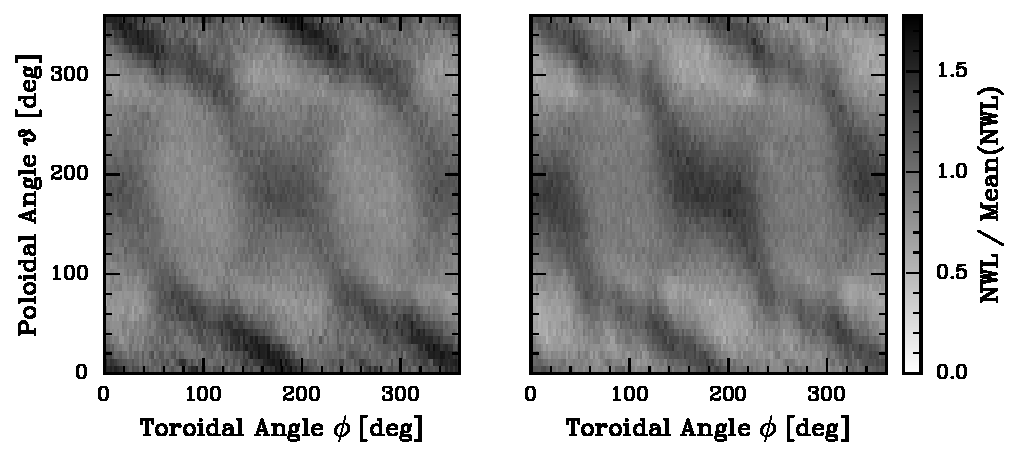
\includegraphics[width=0.95\linewidth]{fig_conformal_map.pdf}
\caption{Neutron wall load $\NWL/\overline{\NWL}$ on the DAGMC conformal first wall of QUASR
device 886079 (real free-streaming \texttt{StellaratorSource} transport): unpolarized
(left) versus peaking-optimal polarization $a_2=+0.82$ (right). The peaking factor falls
only from $1.78$ to $1.49$: the near-field hot spot is not steerable, though the broad load
is visibly redistributed.}
\label{fig:map}
\end{figure}

\begin{figure}[t]
\centering
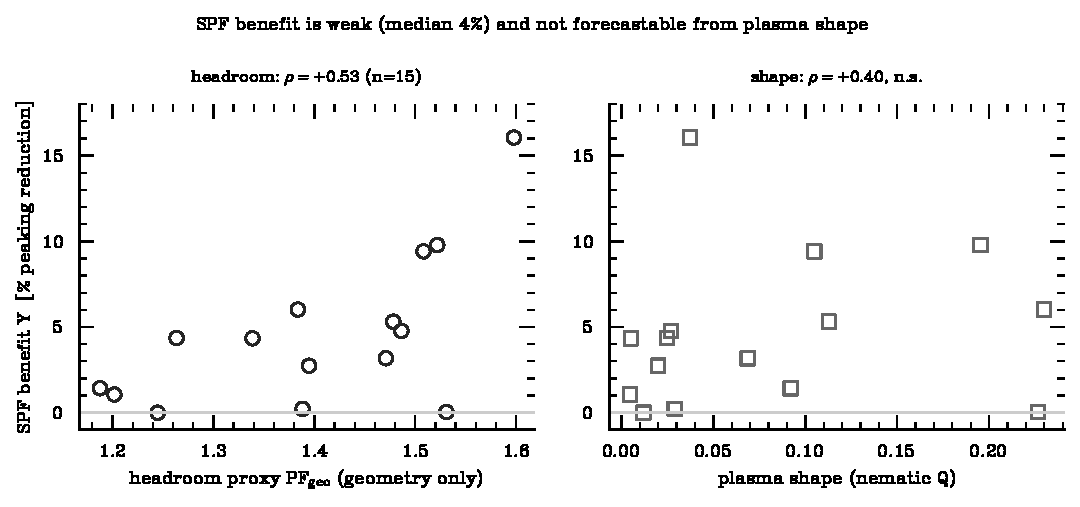
\includegraphics[width=0.90\linewidth]{fig_predictor.pdf}
\caption{The polarization steering benefit is weak and not forecastable from plasma shape
($n=15$ conformal-wall devices). Left: the benefit correlates only weakly with a
transport-free isotropic peaking (headroom) proxy ($\rho=+0.53$, borderline at $n=15$).
Right: it does not correlate with a pure-plasma shape metric ($\rho=+0.40$, not
significant). The steering benefit must be evaluated per device by transport.}
\label{fig:predictor}
\end{figure}

\section{Transported flux and heating on the conformal blanket}
\label{sec:conformalscatter}

Free-streaming isolates the source; a reactor calculation must transport the neutrons through
a real blanket on the real wall. We place the full tungsten / Fe-9Cr steel / beryllium / FLiBe
/ shield / coil blanket conformally on the last-closed surface of device 59509 and mesh it as
a six-material DAGMC solid; because the ARC-class blanket stack is $\sim\!1$~m thick, the
equilibrium is uniformly scaled to a reactor-scale major radius of $\sim\!10$~m (the unit
field $\Bhat$ is scale-invariant, so the polarized emission is unchanged), and the native
\texttt{StellaratorSource} is transported through it with scattering on.
Figure~\ref{fig:cflux} shows the resulting volumetric fast-flux ($E>0.1$~MeV) distribution in
the poloidal plane and the heating deposited in each layer. The fast flux is concentrated in
the plasma-facing region and attenuates through the blanket, and the heating is dominated by
the FLiBe breeder ($84\%$ of the total $1.1\times10^{7}$~eV per source neutron) with the
tungsten first wall taking $\sim\!0.1\%$---the same radial energy partition the box-torus
model of \S\ref{sec:transport} gives, now on the conformal geometry. The near-wall fast flux
itself shifts with the polarization mode at the $\sim\!10\%$ level (perpendicular $-10\%$,
parallel $+10\%$ relative to unpolarized), the anisotropic birth distribution carried through
to the volumetric load. The run exercises the full pipeline end to end on a real device---a
verified VMEC equilibrium, the native polarized source, a conformal multi-material DAGMC
blanket, and scattering transport.

\begin{figure}[t]
\centering
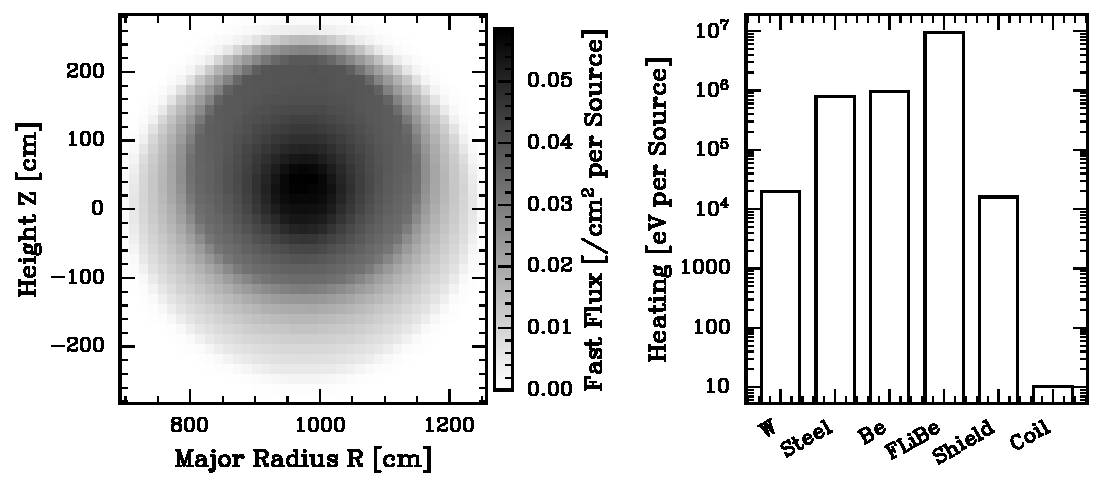
\includegraphics[width=0.95\linewidth]{fig_conformal_flux.pdf}
\caption{Volumetric flux tally on the conformal blanket (device 59509, scattering on, native
\texttt{StellaratorSource}). Left: poloidal fast-flux ($E>0.1$~MeV) distribution
($\phi$-averaged), concentrated in the plasma-facing region and attenuating outward through
the blanket. Right: heating deposited per blanket layer (per source neutron), dominated by
the FLiBe breeder.}
\label{fig:cflux}
\end{figure}

\section{The analytic companion and the division of labour}
\label{sec:companion}

The transport results are cross-checked by, and delimit the validity of, a differentiable
analytic framework for polarized NWL developed in parallel. Its reusable contributions are
three. First, an analytic \emph{singularity subtraction} for the near-singular
free-streaming integral: because the squared source-to-wall distance is a trigonometric
polynomial, the near-singularity's location, depth, and curvature are available in closed
form, so one can subtract an exactly integrable model of the grazing peak and integrate the
smooth remainder with twelve quadrature nodes where fixed Gauss--Legendre needs more than
six thousand, all while remaining automatically differentiable---a construction that
sharpens the singularity-swap approach of af Klinteberg and Barnett~\cite{klinteberg2021}
by obtaining the peak parameters in closed form rather than by root-finding. Second, the
only \emph{polarized} NWL kernels in the analytic literature, riding a differentiable
hybrid quadrature that yields exact geometry gradients---a normalization correction to the
second-order polarized kernel, restoring the unit-field constraint that the leading
derivation drops, advances the polarized series from second to third order. Third, a
characterization of the effective shaping parameter $\epseff$ with two distinct
thresholds---a series-convergence radius near $\tfrac12$ and a larger grazing/quadrature
breakdown near $2$---which quantifies why good quasi-symmetry and geometric near-axisymmetry
anti-correlate, and thereby why the strongly shaped published QAs of \S\ref{sec:validation}
sit in the Monte-Carlo-only regime.

The companion independently reproduces the central result of \S\ref{sec:conformal}: a
single global polarization flattens the full-wall load by under a factor of two, the same
weak-global-lever conclusion the transport reaches, from an entirely separate calculation.
Its native regime is small periodic non-axisymmetry, which maps most honestly not onto
strongly shaped stellarators but onto tokamak toroidal-field ripple, where the wall
signature of the ripple is exponentially suppressed as $e^{-N a/R_0}$ because line-of-sight
integration acts as a low-pass filter on high-harmonic source structure. The two methods
are therefore not competitors but a division of labour: the closed, differentiable analytic
form where the boundary is weakly shaped and gradients drive optimization, and the present
source where the shaping is strong, where the wall is conformal, or where the neutron
transport that the free-streaming methods cannot perform is what a reactor design actually
needs.

\section{Limitations}
\label{sec:limitations}

Several bounds on the present results should be stated. The scattering and rate-trade-off
studies (\S\ref{sec:transport}--\ref{sec:rate}) use a layered box-torus blanket, whose clean
radial geometry isolates the material physics---the $\sim\!3\times$ dilution and the
rate--steering trade-off; the conformal geometry carries the free-streaming load pattern
(\S\ref{sec:conformal}) and the transported volumetric flux and heating
(\S\ref{sec:conformalscatter}). A conformal run resolving the transported inboard/outboard
\emph{steering} would require a first-wall surface-current tally, which the volumetric mesh
of \S\ref{sec:conformalscatter} does not provide; the near-field steering asymmetry is a
surface, not a volumetric, effect. The steering results are monoenergetic at $14.1$~MeV; a
Ballabio-broadened source is available and does not affect the angular physics. The
analytic companion is first-flight and convex-patch, its grazing-robust path is validated
in the unpolarized channel and holds for the polarized channel by construction rather than
by test, and its reverse-mode gradients through the special-function engine do not yet
just-in-time compile. Finally, the conformal-wall study covers fifteen equilibria---enough
to establish that the steering benefit is weak and not forecastable from plasma shape, but
the highly shaped quasi-helical configurations that fail to converge in the fixed-boundary
VMEC solve are under-represented, so the device sample is biased toward the more tractable
quasi-axisymmetric class.

\paragraph{Data availability.}
All numbers, tables, and figures in this paper are reproducible from a self-contained
archive: the frozen transport outputs (the conformal-wall $(\vartheta,\phi)$ load maps, the
scattering and rate ledgers, the fifteen-device predictor table) are stored with a
provenance manifest naming the run that produced each, and one figure script per figure
reads only that archive. The native source, the VMEC producer with its rigor gates, and the
analysis and figure scripts are released with the archive.

\section{Summary}
\label{sec:summary}

We have built and verified the first native, on-the-fly spin-polarized fusion neutron
source in a production Monte-Carlo transport code, realized as an equilibrium-rigorous
\texttt{StellaratorSource}---the first stellarator source, and the first polarized
stellarator source, in OpenMC. The emission kernel separates cleanly into a birth-direction
distribution, sampled exactly by stratification with inverse-CDF draws cross-checked
against rejection, and a scalar rate factor; the sampler reproduces the normalized polarized
kernels to $0.3\%$ with unit mean, and the transported free-streaming loads reproduce the
analytic NWL to $\le1.8\%$ on a real published QA equilibrium, the one $4$--$6\%$ inboard
residual identified by construction as the analytic point-patch limit rather than a defect
of the source. Turning on transport, we find that scattering dilutes the geometric steering
by a factor of $\sim\!3$---a correction only a transport calculation can supply; restoring
the reactivity, we find that the $+50\%$-rate mode compounds the center-stack load to
$1.70\times$ while the equal-rate parallel mode relieves it to $0.85\times$ at no cost to
power or to the tritium breeding ratio; and on conformal first walls of real stellarators we
find that peaking-optimal polarization lowers the peaking factor only modestly because the
load peak is an unsteerable near-field spike, so polarization is a strong local but weak
global actuator---a conclusion an independent differentiable analytic method reaches as
well. The source is available for both tokamak- and stellarator-class equilibria and
provides a verified, honest foundation for polarized-fuel reactor neutronics.

\begin{thebibliography}{99}

\bibitem{schwartz2025}
A.~Schwartz \emph{et al.}, Neutron wall loading for spin-polarized fusion in axisymmetric
geometries, arXiv:2507.11758, 2025.

\bibitem{lion2022}
J.~Lion, F.~Warmer, and H.~Wang, A deterministic method for the fast evaluation and
optimisation of the 3D neutron wall load for generic stellarator configurations,
\emph{Nucl. Fusion} \textbf{62}, 076040 (2022).

\bibitem{parisi2024}
J.~F.~Parisi, A.~Diallo, and J.~A.~Schwartz, Simultaneous enhancement of tritium burn
efficiency and fusion power with low-tritium spin-polarized fuel, \emph{Nucl. Fusion}
\textbf{64}, 126019 (2024).

\bibitem{kulsrud1982}
R.~M.~Kulsrud, H.~P.~Furth, E.~J.~Valeo, and M.~Goldhaber,
Fusion reactor plasmas with polarized nuclei,
\emph{Phys. Rev. Lett.} \textbf{49}, 1248 (1982).

\bibitem{bae2025}
C.~Bae \emph{et al.}, Neutronics analysis of spin-polarized fuel in spherical tokamaks,
\emph{Nucl. Fusion} \textbf{65}, 086051 (2025).

\bibitem{lyytinen2024}
T.~Lyytinen, A.~Snicker, J.~Virtanen, I.~Palermo, J.~Alguacil, T.~Bogaarts, and F.~Warmer,
Proof-of-principle of parametric stellarator neutronics modeling using Serpent2,
\emph{Nucl. Fusion} \textbf{64}, 076042 (2024).

\bibitem{peterson_tokamaksource}
E.~E.~Peterson \emph{et al.}, A parametric tokamak plasma source for OpenMC, OpenMC pull
request \#3999 (2025).

\bibitem{hirshman1983}
S.~P.~Hirshman and J.~C.~Whitson, Steepest-descent moment method for three-dimensional
magnetohydrodynamic equilibria, \emph{Phys. Fluids} \textbf{26}, 3553 (1983).

\bibitem{klinteberg2021}
L.~af~Klinteberg and A.~H.~Barnett, Accurate quadrature of nearly singular line integrals in
two and three dimensions by singularity swapping, \emph{BIT Numer. Math.} \textbf{61}, 83
(2021).

\bibitem{landreman2022}
M.~Landreman and E.~Paul, Magnetic fields with precise quasisymmetry for plasma
confinement, \emph{Phys. Rev. Lett.} \textbf{128}, 035001 (2022).

\bibitem{romano2015}
P.~K.~Romano, N.~E.~Horelik, B.~R.~Herman, A.~G.~Nelson, B.~Forget, and K.~Smith,
OpenMC: A state-of-the-art Monte Carlo code for research and development,
\emph{Ann. Nucl. Energy} \textbf{82}, 90 (2015).

\bibitem{dagmc}
P.~C.~Shriwise, A.~Davis, L.~J.~Jacobson, and P.~P.~H.~Wilson,
Particle tracking acceleration on CAD geometries in DAGMC, 2017.

\bibitem{quasr}
A.~Giuliani \emph{et al.}, QUASR: a database of quasisymmetric stellarators and their
coils, Flatiron Institute; \url{https://quasr.flatironinstitute.org}.

\end{thebibliography}

\end{document}
